\section{Sound, Music and Mathematics}

After learning about (standing)  waves, superposition and harmonics, we now want to understand how these ideas help us describe \textbf{sound and music}. In particular, we will see how mathematical concepts such as sine functions and and physical concepts such as superposition explain why musical instruments produce different sounds.

\subsection{Fundamental Frequency and Harmonics}

When a string (for example on a guitar) vibrates, it does not only oscillate as a whole. Instead, it can vibrate in several different ways at the same time due to superposition.  We will now investigate how this influences the sound we perceive. 

The simplest vibration is called the \textbf{fundamental frequency/natural frequency}. A musical sound can only be perceived if there are standing waves as they show the same vibrating pattern over a period of time. Without standing waves the sound perceived is more likely identified as noise.
The fundamental frequency determines the pitch of the tone we hear. Let us consider a guitar string. It is fixed at both ends. As we have learned in this case, the simplest standing wave that can occur is the 1st harmonic with Node - Antinode - Node. Its wave length is given by $ \lambda = 2 l  \Leftrightarrow l = \lambda/2$ .Using the speed of sound, each wavelength can be converted into a corresponding frequency. 

\begin{align}
    f _1=  \frac{c}{2l}
\end{align}
This frequency is the \textbf{fundamental frequency/natural frequency} of the guitar sting considered. This frequecy determines the pitch we perceive. Thus, if the string is shortened , we perceive a higher tone. 

In addition, the string can also vibrate in smaller sections. As we have learned above, these vibrations are generally called \textbf{harmonics}. If we consider musical instruments we also call these vibrations  \textbf{overtones}.

Mathematically, the frequencies of these harmonics are given by:
\begin{equation}
    f_n = \frac{n \cdot c}{2l}=  n \cdot f_1
\end{equation}

\begin{itemize}
    \item $f_1$: fundamental frequency
    \item $n = 1,2,3,\dots$: harmonic number
\end{itemize}

\paragraph{Intuitive Explanation:}
\begin{itemize}
    \item The string can vibrate as a whole (first harmonic) $\rightarrow $ fundamental frequency $f_1$
    \item It can also vibrate in two halves (second harmonic) $\rightarrow $ first overtone $f_2 = 2 f_1$
    \item Or in three parts, four parts, and so on$\rightarrow $  second / third...  overtone $f_n = n f_1$
\end{itemize}

\begin{table}[h]
\centering
\begin{tabular}{|c|c|c|l|}
\hline
$n$ & Name & Frequency & Pattern on string \\
\hline
1 & Fundamental (1st harmonic) & $f_1$       & N---A---N \\
2 & 2nd harmonic (1st overtone) & $2f_1$     & N-A-N-A-N \\
3 & 3rd harmonic (2nd overtone) & $3f_1$     & N-A-N-A-N-A-N \\
4 & 4th harmonic (3rd overtone) & $4f_1$     & N-A-N-A-N-A-N-A-N \\
\hline
\end{tabular}
\caption{Harmonics of a string fixed at both ends (N = node, A = antinode)}
\label{tab:harmonics}
\end{table}

Each of these vibrations can occur at the same string and  corresponds to a different sine wave and thus to a different frequency. But all those frequencies are described by the correlation $f_n = n \times f_1$. 
To summarize, we need sine and cosine functions to describe standing waves which generate a tone at a specific frequency / pitch. For a specific string there are many standing waves that can occur. 


\paragraph{Concrete Example: Guitar String}
A guitar string has a length of $l = 65\,\text{cm} = 0.65\,\text{m}$. 
The wave speed on the string is approximately $c = 286\,\frac{\text{m}}{\text{s}}$. 
The fundamental frequency is then:
\begin{equation}
    f_1 = \frac{c}{2l} = \frac{286}{2 \cdot 0.65} \approx 220\,\text{Hz}
\end{equation}
This corresponds to the note A3. The harmonics are then at 
$440\,\text{Hz}$ (A4), $660\,\text{Hz}$, $880\,\text{Hz}$ (A5), and so on. 



\subsection{Superposition of Waves and Sound}
We have learned in the last chapter that waves show superposition. This means that even the guitar string can vibrate with different frequencies at the same time. All those frequencies correspond to the one of standing waves we determined before ($f =f_1 \cdot n$). So intuitively, different standing waves (harmonics) overlap.  At each 
point of the string the displacement of the different standing waves add up to the total displacement. The resulting sound is thus a \textbf{superposition} of many sine waves. So, we can describe the motion of the string using the following equation: 
\begin{equation}
    y(x,t) = A_1 \sin(2\pi f_1 t) + A_2 \sin(2\pi f_2 t) + A_3 \sin(2\pi f_3 t) + \ldots
\end{equation}
Here, $A_1, A_2, A_3, \ldots$ are the \textbf{amplitudes} of the individual harmonics. 
They describe how strongly each harmonic is present in the sound.

\paragraph{Key Idea:}
Any periodic sound can be written as a sum of sine and cosine functions. 
This remarkable mathematical fact is known as \textbf{Fourier's theorem}, named after the 
French mathematician Jean-Baptiste Joseph Fourier (1768--1830). It means that no matter how 
complicated a sound wave looks, it can always be broken down into simple sine waves.

This is why the sine function is so fundamental in acoustics: it is the 
\textbf{basic building block} of all sounds.


\paragraph{Visualising Superposition:}
Consider two sine waves with frequencies $f_1$ and $2f_1$:
\begin{align}
    y_1(t) &= \sin(2\pi f_1 t) \\
    y_2(t) &= \frac{1}{2}\sin(2\pi \cdot 2f_1 \cdot t)
\end{align}
Their sum $y_1 + y_2$ already produces a noticeably different wave shape -- 
no longer a pure sine, but a more complex periodic curve. Adding more harmonics 
makes the shape even richer. This is exactly what happens inside a musical instrument. So a specific mixture of the harmonics causes a specific sound. 



\subsection{Timbre: Why Instruments Sound Different}
So far, we have learned that a musical sound is usually a superposition of many sine waves.
The lowest frequency is the \textbf{fundamental frequency}, which determines the pitch.
The higher frequencies are the \textbf{harmonics} (or overtones). However, not every harmonic
has the same amplitude.

\paragraph{The Sound Spectrum} 
The \textbf{sound spectrum} shows which frequencies are contained in a sound and how strong
each of them is. In other words, it tells us which harmonics are present and how large their
amplitudes are.

If we draw the spectrum, the horizontal axis represents the frequency and the vertical axis
represents the amplitude. Every peak in the spectrum corresponds to one harmonic. As you might notice, the frequency is plotted using a logarithmic scale. We will discuss in the following chapters why using this scale is favorable. 


\begin{figure}[!ht]
\begin{center}
   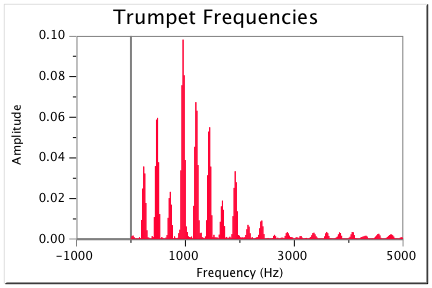
\includegraphics[height = 7 cm ]{Bilder/trumpet.png}
    
    \caption{\footnotesize sound spectrum of a trumpet}
    \label{img: spectrum trumpet}

    %Quelle: https://mind-sized-bites.firebaseapp.com/timbre/timbre.html
\end{center}
\end{figure}



A high peak means that this frequency is very strong in the sound, while a small peak means
that the corresponding harmonic is only weakly present. The fundamental frequency is the peak at the lowest frequency and is thus the frequency which we perceive as pitch. All the other frequencies contained in the sound do  not change the pitch; instead, they determine the sound or timbre of the instrument. In \autoref{img: spectrum trumpet} you can see a sound spectrum of a trumpet. 

\paragraph{What is Timbre?}

Two instruments can play exactly the same note, meaning they have the same
\textbf{fundamental frequency}. Nevertheless, they often sound completely different.
For example, you can easily hear the difference between a piano, a guitar and a flute,
even if they all play the same note.
This difference is called the \textbf{timbre} (or tone colour) of an instrument.

The reason is that every instrument produces a different, specific combination of harmonics.
Although the fundamental frequency is the same, the amplitudes of the higher harmonics
are different. Therefore, every instrument has its own characteristic sound spectrum. 
  

\begin{figure}[!ht]
\begin{center}
   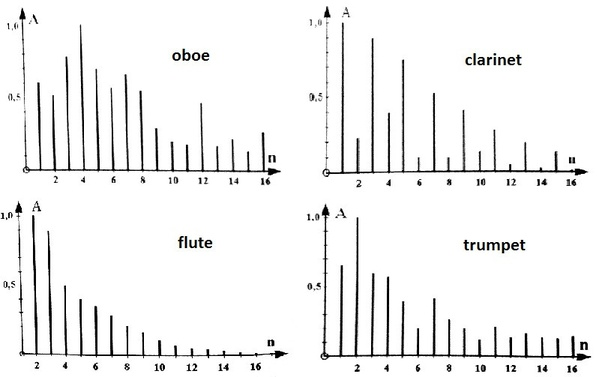
\includegraphics[height = 7 cm ]{Bilder/overtones-of-different-instruments.jpg}
    
    \caption{\footnotesize sound spectra of different instruments at the same fundamental frequency}
    \label{img: sound spectra different instruments }

    %Quelle: 
\end{center}
\end{figure}
In \autoref{img: sound spectra different instruments } you can see the characteristic sound spectra of four different instruments. 


\paragraph{Example}

Suppose a flute and a guitar both play the note A with a fundamental frequency of
$220\,\mathrm{Hz}$.

\begin{itemize}
    \item A \textbf{flute} produces a very strong fundamental frequency and only a few weak harmonics. Its spectrum therefore has one large peak and only small additional peaks. The sound is smooth and pure.
    \item A \textbf{guitar} produces many stronger harmonics. Its spectrum contains several large peaks, making the sound richer and warmer.
\end{itemize}

Even though both instruments play the same pitch, their spectra are different.
Our ears can recognise these differences immediately. This is why we can distinguish
between different musical instruments without even seeing them.

\paragraph{Key Idea}

The \textbf{pitch} of a sound is determined by the fundamental frequency.

The \textbf{timbre} of a sound is determined by the amplitudes of its harmonics, that is, by its sound spectrum.
